In this chapter we will be discussion and showing different results that were obtained while doing simulation and experimentation in both real devices and emulation .

\section{Clock Estimators}

 $$a_{i} = \frac{S \sum^{J_{i}}_{j=1}(\sum^{K_{j}}_{k=1}t_{jK}^{i}.t^{i}_{j}) - \sum^{J_{i}}_{j=1}(\sum^{K_{j}}_{k=1}(t_{jK}^{i})) * \sum^{K_{J_{i}}}_{i=1}(t_{j}^{i}* k_{i})}{S \sum^{J_{i}}_{j=1}(\sum^{K_{j}}_{K=1} (t_{i}^{j})^{2}) - (\sum_{j=1}^{J_{i}}(\sum^{K_{j}}_{K=1} t_{i}^{j}))}
         $$


$$ b_{i} =  \frac{1}{S} [ \sum_{j=1}^{J_{i}}(\sum_{K=1}^{K_{j}} t_{j_{k}}^{i}) - a_{i} * \sum_{j=1}^{J_{i}}(\sum_{K=1}^{K_{j}}t_{j}^{i}.K_{i}) ]$$
\section{Programming Language}
\subsection{C}
C is a general-purpose, imperative computer programming language, supporting structured programming, lexical variable scope and recursion, while a static type system prevents many unintended operations.
\section{Tools}
\subsection{Clion}
Smart C and C++ editor,Thanks to native C and C++ support, including modern C++ standards, libc++ and Boost, CLion knows your code through and through and takes care of the routine while you focus on the important things.
\subsection{Cmake}
CMake is a cross-platform free and open-source software for managing the build process of software using a compiler-independent method. It supports directory hierarchies and applications that depend on multiple libraries.
\subsection{Git}
Git is a free and open source distributed version control system designed to handle everything from small to very large projects with speed and efficiency. Git is easy to learn and has a tiny footprint with lightning fast performance.

\section{Devices}
\subsection{Raspberry}
A Raspberry Pi is a credit card-sized computer originally designed for education, inspired by the 1981 BBC Micro. Creator Eben Upton's goal was to create a low-cost device that would improve programming skills and hardware understanding at the pre-university level.
\subsection{Arduino}
Arduino is an open source computer hardware and software company, project, and user community that designs and manufactures single-board microcontrollers and microcontroller kits for building digital devices and interactive objects that can sense and control objects in the physical and digital world
\section{Emulator}
\subsection{Qemu}
QEMU is a generic and open source machine emulator and virtualizer. Screenshot: QEMU running the ReactOS operating system on Linux. Full-system emulation. Run operating systems for any machine, on any supported architecture.


\section{Basic Arithmetic Operations Timing}
In this section we will be showing time consumation for the basic arithmetic operations depending on the number of digits of operands .

\section{Estimator Calculation Timing}
In this section we will be showing time consumation for calculating the estimator in function of number length
\begin{figure} 
   % \subsection{Raspberry result}

	\hfill
	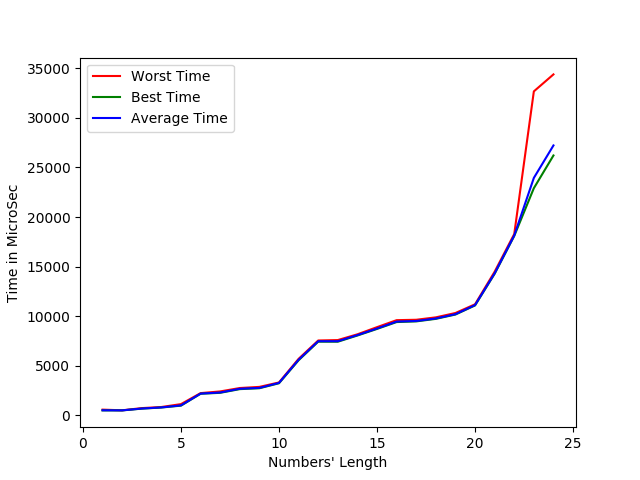
\includegraphics[scale=0.5,width=12cm,height=5cm]{result/raspberry_res.png}
	\caption{Raspberry estimator calculation time}
	\centering
	\label{fig:x raspberry_res}
	\hspace*{\fill}
\end{figure}

\begin{figure} 
   % \subsection{arduino result}

	\hfill
	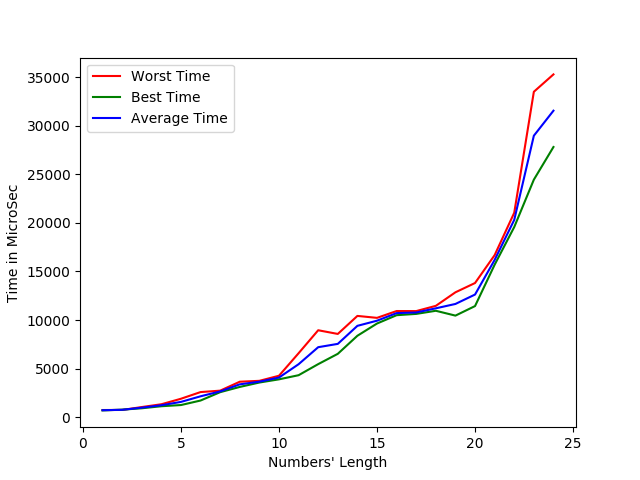
\includegraphics[scale=0.5,width=12cm,height=5cm]{result/arduino_res.png}
	\caption{Arduino estimator calculation time}
	\centering
	\label{fig:x arduino_res}
	\hspace*{\fill}
\end{figure}

\begin{figure} 
   % \subsection{pc result}

	\hfill
	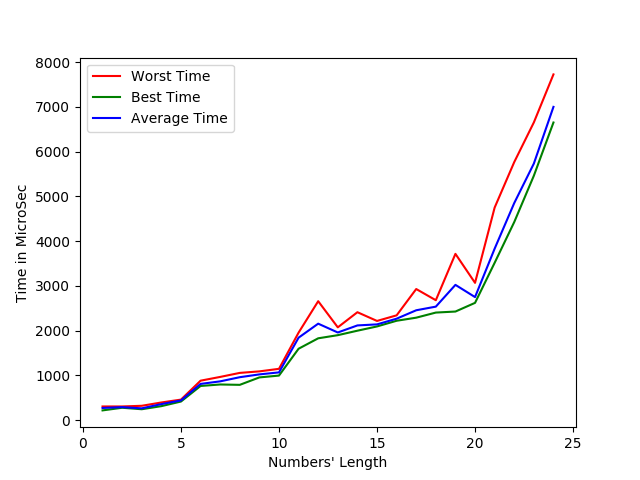
\includegraphics[scale=0.5,width=12cm,height=5cm]{result/pc_res.png}
	\caption{Pc estimator calculation time}
	\centering
	\label{fig:x pc_res}
	\hspace*{\fill}
\end{figure}